% Owner: Keito
\subsubsection{Page layout}
\label{sec:vis-layout}
The page is divided into three columns (Figure~\ref{fig:vis-layout}), with widths in the
ratio 1.15\,:\,3\,:\,2. The left column holds the input and the settings: loading a
recording, the list of loaded recordings (\emph{runs}) and their state, the channel
selection, the heatmap settings, the detection parameters with the \emph{Detect peaks}
button, and the display settings. The centre column holds the two time plots, the
overview of the whole recording and the detail window below it. The right column holds
the activity heatmap and the results: the selected piece, the list of pieces and the
detection summary. Settings, plots and results are thus always in the same place, and
the plots get the widest column.

Each area of the page is one module in \texttt{panels/}, and \texttt{app.py} only places
these modules in the columns. Everything that must survive Streamlit's re-runs, such as
the loaded runs, the detection results, the viewing window and the selected piece, is
kept in \texttt{state.py}, so the panels do not exchange data directly.

Detection algorithms are kept apart from the interface. An algorithm is registered in
\texttt{detectors.py} as a function with a list of parameters, each with a default value
and optional limits. The left column builds a control for every parameter from the type
of its default (slider, number field, check box or text field), and every algorithm
returns the same \texttt{Detection} result, a table of events with at least the columns
\texttt{t\_peak}, \texttt{amplitude}, \texttt{valid} and \texttt{label}. The plots, the
heatmap and the event list therefore work with any algorithm, and a new one needs no
interface code. At present only the pipeline of Sections~\ref{sec:detection-methods}
and~\ref{sec:amount-methods} is registered.

The three columns are limited to the height of the browser window and scroll
independently. When the list of pieces or the settings grow long, the user can scroll
through them while the plots stay in view.

\begin{figure}[H]
  \centering
  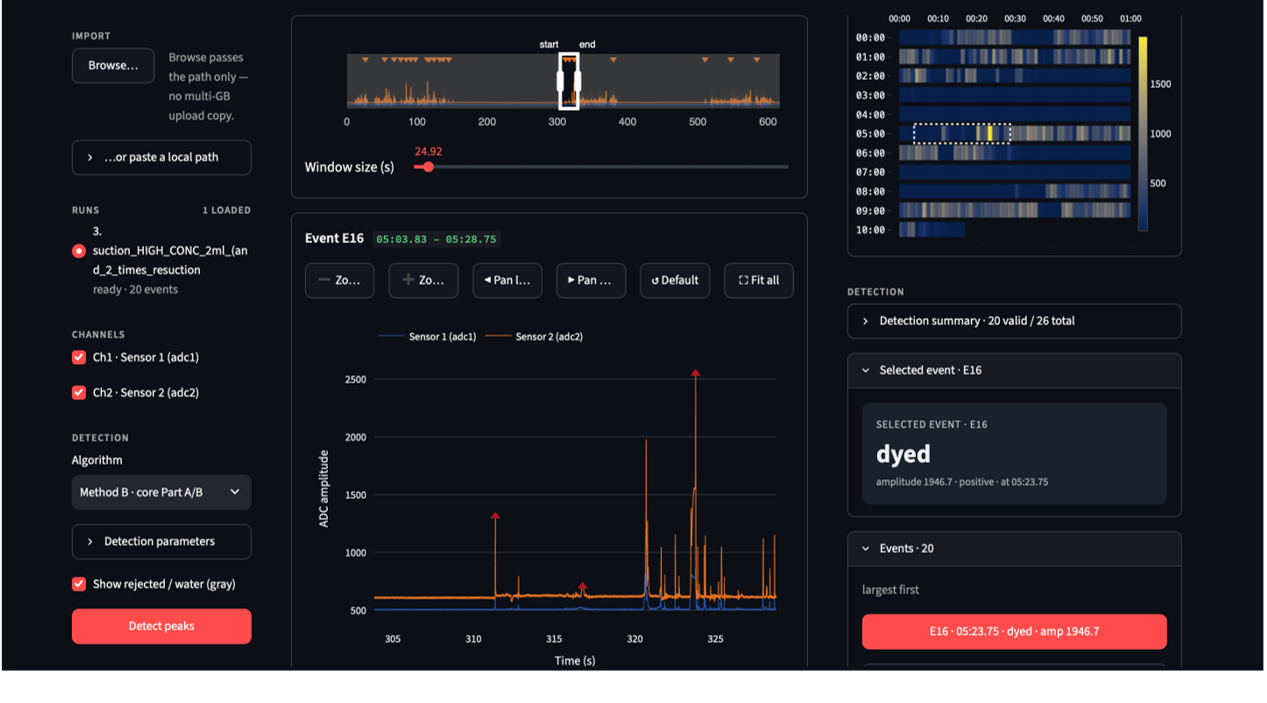
\includegraphics[width=\linewidth]{../images/viewer.png}
  % TODO (Keito): replace with an annotated screenshot (left / centre / right marked).
  \caption{The visualizer. Left: loading and settings. Centre: overview of the whole
           recording with the viewing window, and the detail window. Right: activity
           heatmap and the detected pieces.}
  \label{fig:vis-layout}
\end{figure}
